\documentclass[10pt]{article}
\usepackage[letterpaper,margin=0.66in]{geometry}
\usepackage{amsmath,amssymb,bm}
\usepackage{booktabs,array,multirow}
\usepackage{graphicx}
\usepackage{caption}
\usepackage{enumitem}
\usepackage{multicol}
\usepackage{tikz}
\usepackage{fancyhdr}
\usepackage[hidelinks]{hyperref}
\usepackage{lastpage}
\setlength{\parindent}{0pt}
\setlength{\parskip}{4.2pt}
\setlist[itemize]{leftmargin=*,topsep=2pt,itemsep=1pt,parsep=0pt}
\setlist[enumerate]{leftmargin=*,topsep=2pt,itemsep=1pt,parsep=0pt}
\captionsetup{font=small,labelfont=bf}
\pagestyle{fancy}
\fancyhf{}
\lhead{Walkalong Glider Final Report}
\rhead{ES 220}
\cfoot{\thepage\ of \pageref{LastPage}}
\newcommand{\Rey}{\mathrm{Re}}
\newcommand{\dd}{\mathrm{d}}
\newcommand{\half}{\tfrac{1}{2}}
\newcommand{\placeholder}[2]{\begin{center}\fbox{\begin{minipage}[c][#1][c]{0.9\linewidth}\centering #2\end{minipage}}\end{center}}
\newcommand{\pagehead}[1]{\section*{#1}\addcontentsline{toc}{section}{#1}}
\begin{document}

% PAGE 1
\begin{center}
{\LARGE \textbf{Walkalong Glider}}\\[3pt]
{\large An Investigation of Aerodynamics and Stability in Low Reynolds Number Flight}\\[8pt]
{\normalsize ES 220 Final Project Report}\\[4pt]
{\normalsize Team: \underline{Shriman Jha \& Jackson Shelby} \hspace{0.5in}}
\end{center}

\vspace{2pt}
\begin{abstract}
A walkalong glider is a very light, unpowered airfoil that can remain aloft in a user-generated flow field at approximately walking speed. Unlike a conventional thrown glider, its useful operating state is not free flight through still air; it is flight in a moving flow produced when a person walks behind a board, hand, or other lifting surface. This project studied how such a simple foam aircraft can maintain lift and stability at low speed, where the Reynolds number is low enough that viscous effects, separation, and small geometric changes strongly influence performance. We combined hand analysis, physical prototyping, video-based measurements, and COMSOL simulations to connect observed flight behavior to lift, drag, pitching moment, roll stability, and flow attachment.
\end{abstract}

\textbf{Central question.} How can a nearly massless foam glider sustain stable flight at walking speed, and which geometric parameters make the difference between a glider that follows the walking upwash and one that stalls, dives, rolls, or outruns the user?

\textbf{Main findings.} The working model required an integrated set of design choices rather than one isolated feature. Low mass reduced the required lift and kept the flight speed walkable. A forward center of mass improved pitch stability. Rear camber supplied nose-up trim. Dihedral and a low center of mass improved roll recovery. A downward-tilted or locally aligned leading region helped keep the flow attached and delayed separation. Experimentally, the final light glider had mass $m=0.94$ g, projected area $S=0.011$ m$^2$, flight speed $V=2.2$ m/s, and glide angle satisfying $\tan\gamma=18/90=0.20$. From these measurements, the estimated coefficients were approximately $C_L=0.265$ and $C_D=0.0531$. A heavier model, $m=1.68$ g, flew faster and with higher drag, making it difficult to support at walking speed.


\pagehead{1. Concept and Project Questions}

\subsection*{1.1 What is a walkalong glider?}
A walkalong glider is a lightweight, unpowered airfoil designed to maintain fligh inside a flow field generated by a walking person.The hands, head, or board held by the user deflects incoming air upward relative to the glider, creating an upwash region. The glider does not contain propulsion; its equilibrium force balance is maintained by continuously moving through the user-generated flow field.

The useful distinction is between \textit{unforced glide} and \textit{forced walkalong flight}. In unforced glide, the glider trades height for forward motion and descends at a glide angle $\gamma$. In forced walkalong flight, the incoming air has a vertical component induced by the walking object. The glider can then remain near constant height relative to the user if the induced vertical flow balances the natural sink rate.

\subsection*{1.2 How does it work?}
The glider works by combining ordinary lift generation with very low wing loading. Because its weight is small, the required lift force is also small. The pressure difference across the wing and the momentum deflection of air can therefore support the glider at speeds close to walking speed. The walking object supplies an effective upward component of relative wind. To stay with the user, the glider must have a trim speed low enough that the walking flow can keep up with it, and a sink speed low enough that the upwash can replace lost gravitational potential energy.

\subsection*{1.3 Main principles}
The project reduced to four coupled principles.
\begin{enumerate}
\item \textbf{Low wing loading:} Lower mass and larger area reduce the required dynamic pressure and lift so the glider can fly slowly.
\item \textbf{Pitch trim and pitch stability:} A forward center of mass and rear camber allow a positive angle of attack without uncontrolled pitch-up.
\item \textbf{Roll stability:} Dihedral makes a banked glider generate more restoring lift on the lower wing; a low center of mass adds pendulum-like recovery.
\item \textbf{Separation control:} A locally aligned leading edge and suitable nose tilt reduce adverse separation and flutter at low Reynolds number.
\end{enumerate}

\subsection*{1.4 What do we gain by studying it?}
The system is useful because it exposes low-speed aerodynamics without requiring a wind tunnel or powered aircraft. It also creates a compact testbed for stability: geometry changes that seem small, such as a slight nose tilt or trailing-edge camber, produce immediately visible changes in flight. The result is a physical demonstration of how lift, drag, moments, Reynolds number, and flow attachment interact in an underactuated flying system.



% PAGE 3
\pagehead{2. Aerodynamic Theory}

\subsection*{2.1 Lift, drag, and glide equilibrium}
For a glider in steady, unforced descent, lift acts approximately perpendicular to the flight path and drag acts opposite the flight path. If $\gamma$ is the glide angle below horizontal, force balance gives
\begin{equation}
L = mg\cos\gamma, \qquad D = mg\sin\gamma, \qquad \frac{D}{L}=\tan\gamma
\end{equation}
The aerodynamic forces are written using dimensionless coefficients:
\begin{equation}
L = \frac{1}{2}\rho V^2 S C_L, \qquad D = \frac{1}{2}\rho V^2 S C_D,
\end{equation}
where $\rho$ is air density, $V$ is airspeed, $S$ is projected planform area, $C_L$ is the lift coefficient, and $C_D$ is the drag coefficient. Combining these equations gives the data-reduction formulas used in the experiment:
\begin{equation}
C_L = \frac{2mg\cos\gamma}{\rho V^2 S}, \qquad C_D = \frac{2mg\sin\gamma}{\rho V^2 S}.
\end{equation}
These equations also show why weight dominated the design process. At fixed $S$, $C_L$, and air density, the required trim speed scales as
\begin{equation}
V \sim \sqrt{\frac{2mg\cos\gamma}{\rho S C_L}}.
\end{equation}
A heavier glider must either fly faster, fly at higher $C_L$, or descend more steeply. For walkalong flight, all three options are costly: higher speed outruns the user, higher $C_L$ increases separation risk, and a steeper sink angle demands more upwash.

\subsection*{2.2 Forced-flow interpretation}
In walkalong flight, the relative flow is not simply the negative of the glider velocity through still air. Let $\mathbf{v}_g$ be the glider velocity and let $\mathbf{u}_w(\mathbf{r},t)$ be the local flow velocity produced by the walking object. The air-relative velocity is
\begin{equation}
\mathbf{V}_{rel}=\mathbf{v}_g-\mathbf{u}_w(\mathbf{r},t), \qquad V_{rel}=\|\mathbf{V}_{rel}\|.
\end{equation}
The walking object is useful when $\mathbf{u}_w$ has an upward component at the glider. This effectively reduces the required sink rate. If the natural unforced sink speed is $V\sin\gamma$, a simple condition for approximately level walkalong flight is
\begin{equation}
u_w \gtrsim V\sin\gamma,
\end{equation}
where $u_w$ is the upward component of the induced flow. This is not a complete flow model, but it captures the key requirement: the user does not eliminate gravity; the user supplies a flow field that compensates for the glider's sink.

\subsection*{2.3 Angle of attack and local geometry}
The lift and moment depend on angle of attack, $\alpha$, the angle between the chord reference line and the local relative wind. The challenge is that the local flow direction changes along the wing and with the user's walking motion. The glider therefore benefits from geometric features that create acceptable local angles of attack across the surface. Rear camber raises the aft portion of the airfoil and helps create a nose-up moment, while nose tilt can align the leading surface with the incoming flow and reduce early separation.


% PAGE 4
\pagehead{3. State-Vector Equations of Motion}

To model the walk-along glider, we treated the glider as a lightweight rigid body moving in a vertical plane. The body-frame velocity components are \(u\), along the chord, and \(w\), normal to the chord. The pitch angle is \(\theta\), the pitch rate is \(q=\dot{\theta}\), and the inertial position is \((x_g,z_g)\). The derivation first writes the still-air glider dynamics, then modifies the relative airflow when the walker introduces an upwash field. Thus, the walker does not apply a direct mechanical force; it changes the effective velocity, angle of attack, lift, drag, and moment.

\begingroup
\small
\setlength{\jot}{3pt}

\[
\textbf{Unforced state vector:}
\qquad
\mathbf{x}_0 =
\begin{bmatrix}
u & w & q & x_g & z_g & \theta
\end{bmatrix}^{T}
\]

\begin{align}
\dot{u} &= wq + \frac{1}{m}\left[X_0 - mg\sin\theta\right],
&
\dot{w} &= -uq + \frac{1}{m+M_{33}}\left[Z_0 + mg\cos\theta\right],
&
\dot{q} &= \frac{M_0}{I_{\mathrm{eff}}}, \\
\dot{x}_g &= u\cos\theta - w\sin\theta,
&
\dot{z}_g &= u\sin\theta + w\cos\theta,
&
\dot{\theta} &= q.
\end{align}

\[
\textbf{Forced state vector:}
\qquad
\mathbf{x}_f =
\begin{bmatrix}
u & w & q & x_g & z_g & \theta & x_w
\end{bmatrix}^{T}
\]

\begin{align}
\dot{u} &= wq + \frac{1}{m}\left[X_0+\Delta X_w - mg\sin\theta\right],
&
\dot{w} &= -uq + \frac{1}{m+M_{33}}\left[Z_0+\Delta Z_w + mg\cos\theta\right],
&
\dot{q} &= \frac{M_0+\Delta M_w}{I_{\mathrm{eff}}}, \\
\dot{x}_g &= u\cos\theta - w\sin\theta,
&
\dot{z}_g &= u\sin\theta + w\cos\theta,
&
\dot{\theta} &= q,
\qquad
\dot{x}_w = V_w(t).
\end{align}

The aerodynamic force components are written as

\begin{align}
X_j &= -D_j\cos\alpha_j + L_j\sin\alpha_j,
&
Z_j &= -L_j\cos\alpha_j - D_j\sin\alpha_j,
&
j &\in \{0,\mathrm{rel}\},
\end{align}

where

\begin{align}
L_j &= \frac{1}{2}\rho_f S V_j^2 C_L(\alpha_j),
&
D_j &= \frac{1}{2}\rho_f S V_j^2 C_D(\alpha_j).
\end{align}

For still air,

\begin{align}
V_0 &= \sqrt{u^2+w^2},
&
\alpha_0 &= \theta + \tan^{-1}\left(\frac{w}{u}\right).
\end{align}

For the forced walk-along case, the wind-relative velocity is

\begin{align}
u_{\mathrm{rel}} &= u-u^B_{\mathrm{ind}},
&
w_{\mathrm{rel}} &= w-w^B_{\mathrm{ind}},
&
V_{\mathrm{rel}} &= \sqrt{u_{\mathrm{rel}}^2+w_{\mathrm{rel}}^2},
&
\alpha_{\mathrm{rel}} &= \theta+\tan^{-1}
\left(\frac{w_{\mathrm{rel}}}{u_{\mathrm{rel}}}\right).
\end{align}

The walker-induced aerodynamic increments are

\begin{align}
\Delta X_w &= X_{\mathrm{rel}}-X_0,
&
\Delta Z_w &= Z_{\mathrm{rel}}-Z_0,
&
\Delta M_w &= M_{\mathrm{rel}}-M_0.
\end{align}

\[
\boxed{
\text{Forced dynamics}
=
\text{unforced dynamics}
+
\text{walker-induced aerodynamic increments}.
}
\]

\endgroup
\newpage

% PAGE 5
\pagehead{4. Reynolds Number and Regime Characterization}

\subsection*{4.1 What Reynolds number means}
The Reynolds number compares inertial forces to viscous forces:
\begin{equation}
\Rey=\frac{\rho V c}{\mu}=\frac{Vc}{\nu},
\end{equation}
where $c$ is the characteristic length, usually mean chord for an airfoil, $\mu$ is dynamic viscosity, and $\nu$ is kinematic viscosity. The Reynolds number is a useful indicator of the flow regime, specifically when the flow can turn from laminar to turbulent. Low Reynolds number flight is difficult because the boundary layer has less momentum near the wall and is more likely to separate under an adverse pressure gradient. For this project, small changes in nose shape, camber, angle of attack, and surface roughness can cause large differences in glide behavior.

\subsection*{4.2 Comparison to other flyers}

Using $V=1.5 - 3$ m/s and a representative chord $c=0.05$--$0.10$ m gives
\begin{equation}
\Rey \approx \frac{(1.5 \text{ to } 3)(0.05\text{ to }0.10)}{1.5\times 10^{-5}} \approx 5\times 10^3\text{--}2\times 10^4.
\end{equation}

\begin{center}
\begin{tabular}{lccc}
\toprule
System & Typical speed scale & Length scale & Approximate $\Rey$ scale \\
\midrule
Small insects / tiny indoor flyers & very low & millimeters-cm & $10^2$-$10^4$ \\
Walkalong glider & walking speed & cm-scale chord & $10^3$-$10^4$  \\
Birds / small UAVs & moderate & cm-m scale & $10^5$ \\
Commercial aircraft & high & m scale & $10^6$-$10^7$ or higher \\
\bottomrule
\end{tabular}
\end{center}




\subsection*{4.3 Design considerations based on Re regime}

Experiments show that typically around Re on the order of $10^5$ the flow transitions from laminar to turbulent. On the scale of our glider the Reynolds number is lower and so flow is mostly laminar. However, locally the flow can have a higher Re and become turbulent. This unsteadiness of the flow can cause problems for our gliders stability, causing observable effects like gliders that glide for a short period before losing lift and plummeting out of the air. Furthermore, the viscous boundary layer over the wings has low momentum in this regime, and can separate easily. This separation may lead to the turbulence mentioned before. It is therefore crucial to consider in the design of a glider, adjustments and changes that may reduce the unsteady risks associated with separation and turbulence. 

\newpage

% PAGE 6
\pagehead{5. Experimental Build and Design Evolution}

\subsection*{5.1 What we built}
The final prototype was a foam walkalong glider made from lightweight expanded polystyrene (EPS) sheet material. The stock material was cut down to 1mm in thickness with a hot-wire foam cutter. The geometry was shaped by cutting and bending the foam to create a thin cambered airfoil with dihedral. A length of Nitinol wire was taped to the nose to set the center of mass ahead of the aerodynamic center. The final measured mass was
\begin{equation}
m=0.94\text{ g}=9.4\times10^{-4}\text{ kg}, \qquad S=0.011\text{ m}^2.
\end{equation}

\begin{figure}[h!]
    \centering

    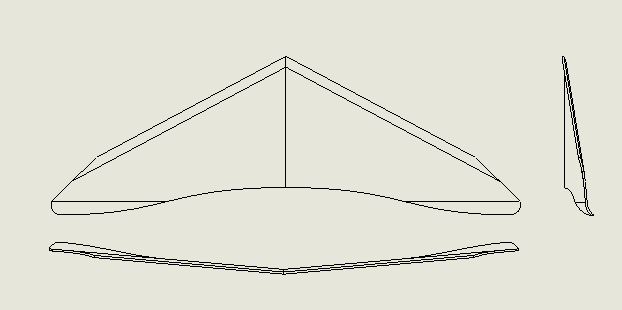
\includegraphics[width=1\linewidth]{Screenshot 2026-05-08 154735.png}
    \caption{Top, front and side view of the glider}

\end{figure}

\subsection*{5.2 Build process and design choices}
The build process was iterative. Initial versions were evaluated by hand launch and by walking behind a large surface to produce upwash. Designs were modified when they showed one of four failure modes: rapid nose-down dive, pitch-up stall, roll-off to one side, or inability to remain in the upwash without excessive walking speed. The successful design emerged from reducing weight and tuning stability features rather than from simply increasing wing area.

\subsubsection*{5.21 Weight and wing loading}

As discussed earlier, it is readily apparent from the dynamical equations that reducing mass per unit wing area is very important. To recap simply, more weight requires more Lift to balance gravity, more lift requires a higher velocity or steeper glide, and we need a slow glider with a gentle glide ratio to fly. Materials such as paper and parchment proved insufficient both in weight and in structural stability. A few different foam materials varying in density strength were tested, which the conclusion that EPS is one of the few that was both light enough and also sturdy enough. A 1mm section was cut from 3mm stock (cafeteria treys ordered on Amazon). In addition, we chose a wire for the front weight, as the ability to use less mass, further from the airfoil, rather than more mass, closer to the foil allowed for further weight minimization. 

\subsubsection*{5.22 Roll stability}

Two specific design choices were made in regards to the roll stability of the aircraft. The first is a low center of mass, which was added by directing the added front weight down at an angle. 

\begin{figure}[h!]
    \centering
    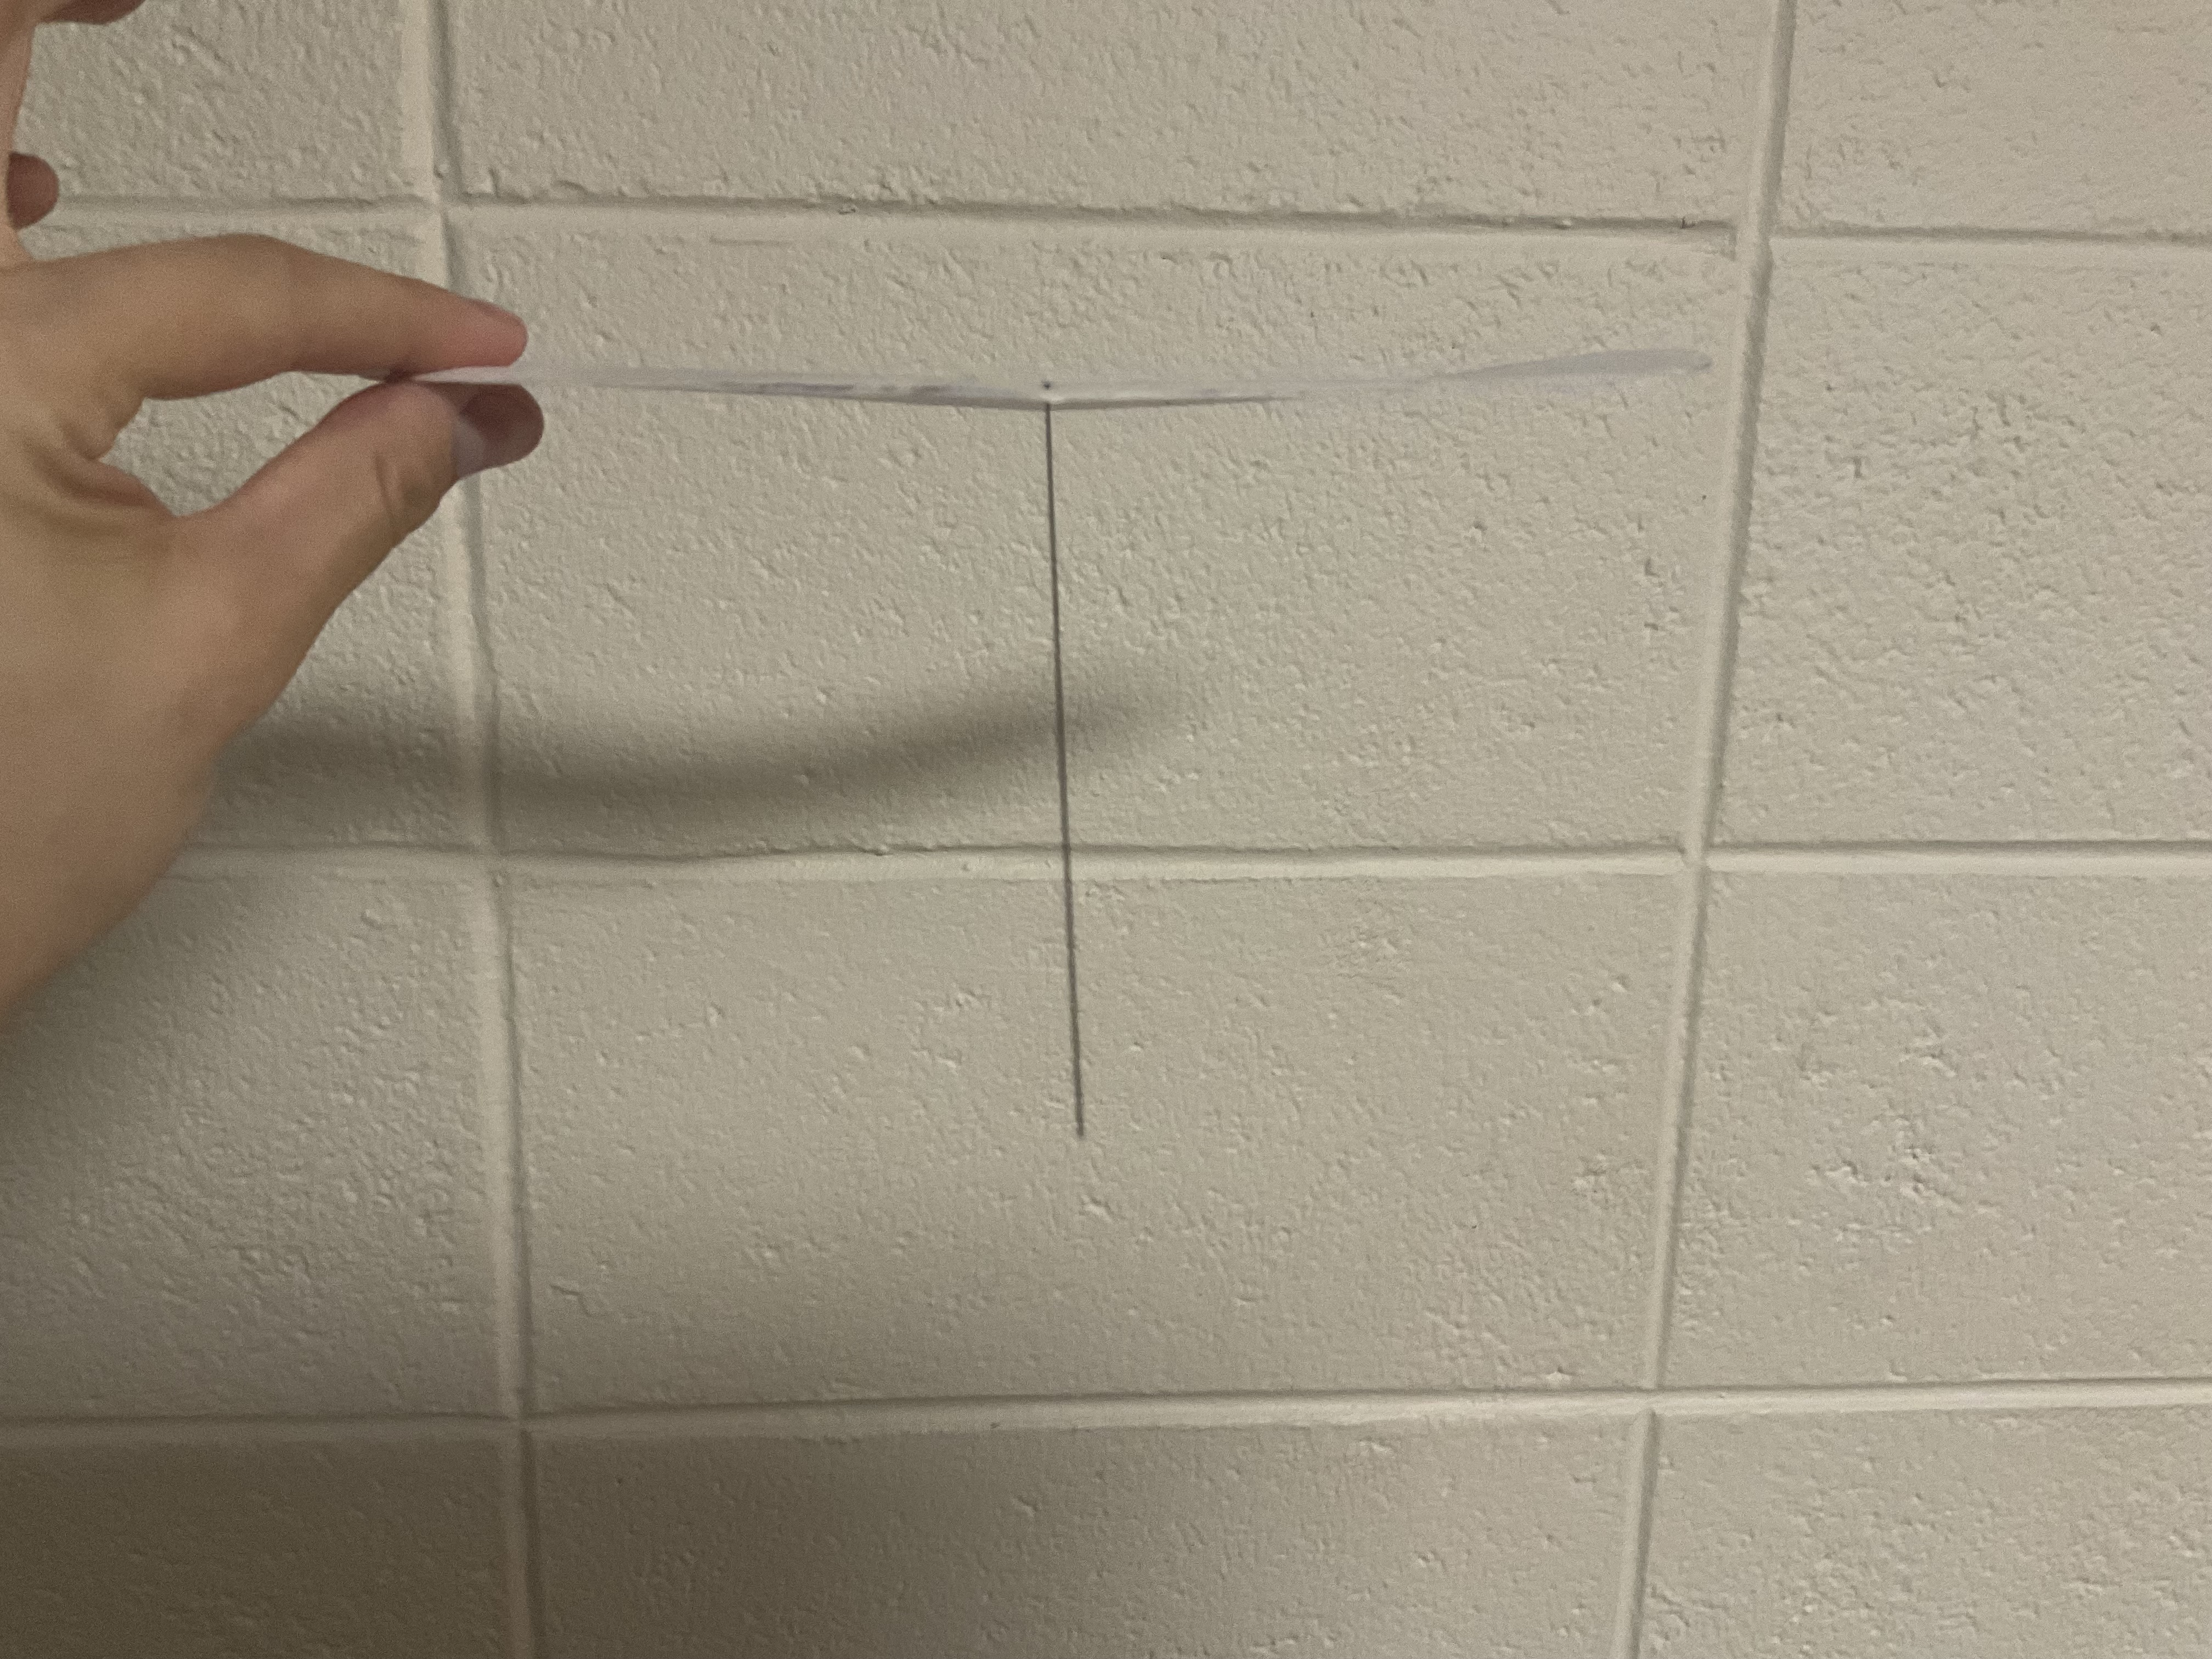
\includegraphics[width=0.5\linewidth]{IMG_3465.jpg}
    \caption{front weight hangs down below glider}
    \label{fig:placeholder}
\end{figure}

Obviously, with a CoM, above the wings, the glider wants to flip over, in order for its center of mass to be lower and for it to reduce potential energy, so it would be unstable. The low CoM acts like a pendulum, with damping from the wings: it applies a restoring torque to reduce roll when offset from equilibrium. Mathematically:

\begin{equation}
M_{roll, CoM} = -mgh\sin \theta \approx -mgh\theta
\end{equation}

Where $\theta$ is the roll angle

The other design consideration for roll stability is the dihedral.

\begin{figure}[h!]
    \centering
    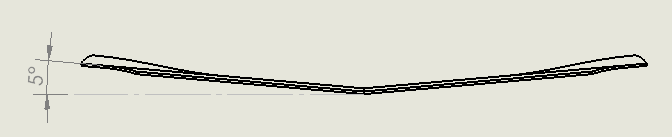
\includegraphics[width=0.7\linewidth]{Screenshot 2026-05-08 164713.png}
    \caption{Dihedral angle}
    \label{fig:placeholder}
\end{figure}


 The wings are both tilted up a few degrees above the horizontal. When the glider rolls clockwise, for example, the projected surface area of the right wing onto the horizontal increases while that of the left wing decreases. This applies a restoring torque. Mathematically:

\begin{equation}
 M_{roll, Dihedral} = \frac{1}{2}\rho V^{2}A\cos(\theta+\theta_0)\times l - \frac{1}{2}\rho V^{2}A\cos(-\theta+\theta_0)\times l
\end{equation}

Where A is the wing area, $\theta_0$ is the dihedral angle, $\theta$ is the roll angle, and $l$ is some length from where the lift acts to the center of the two wings. 

\newpage

\subsubsection*{5.23 Pitch Stability}

There were also two specific design considerations made to ensure that the glider maintained an even pitch. The first is to move the CoM forwards with respect to the aerodynamic center.

\begin{figure}[h!]
    \centering
    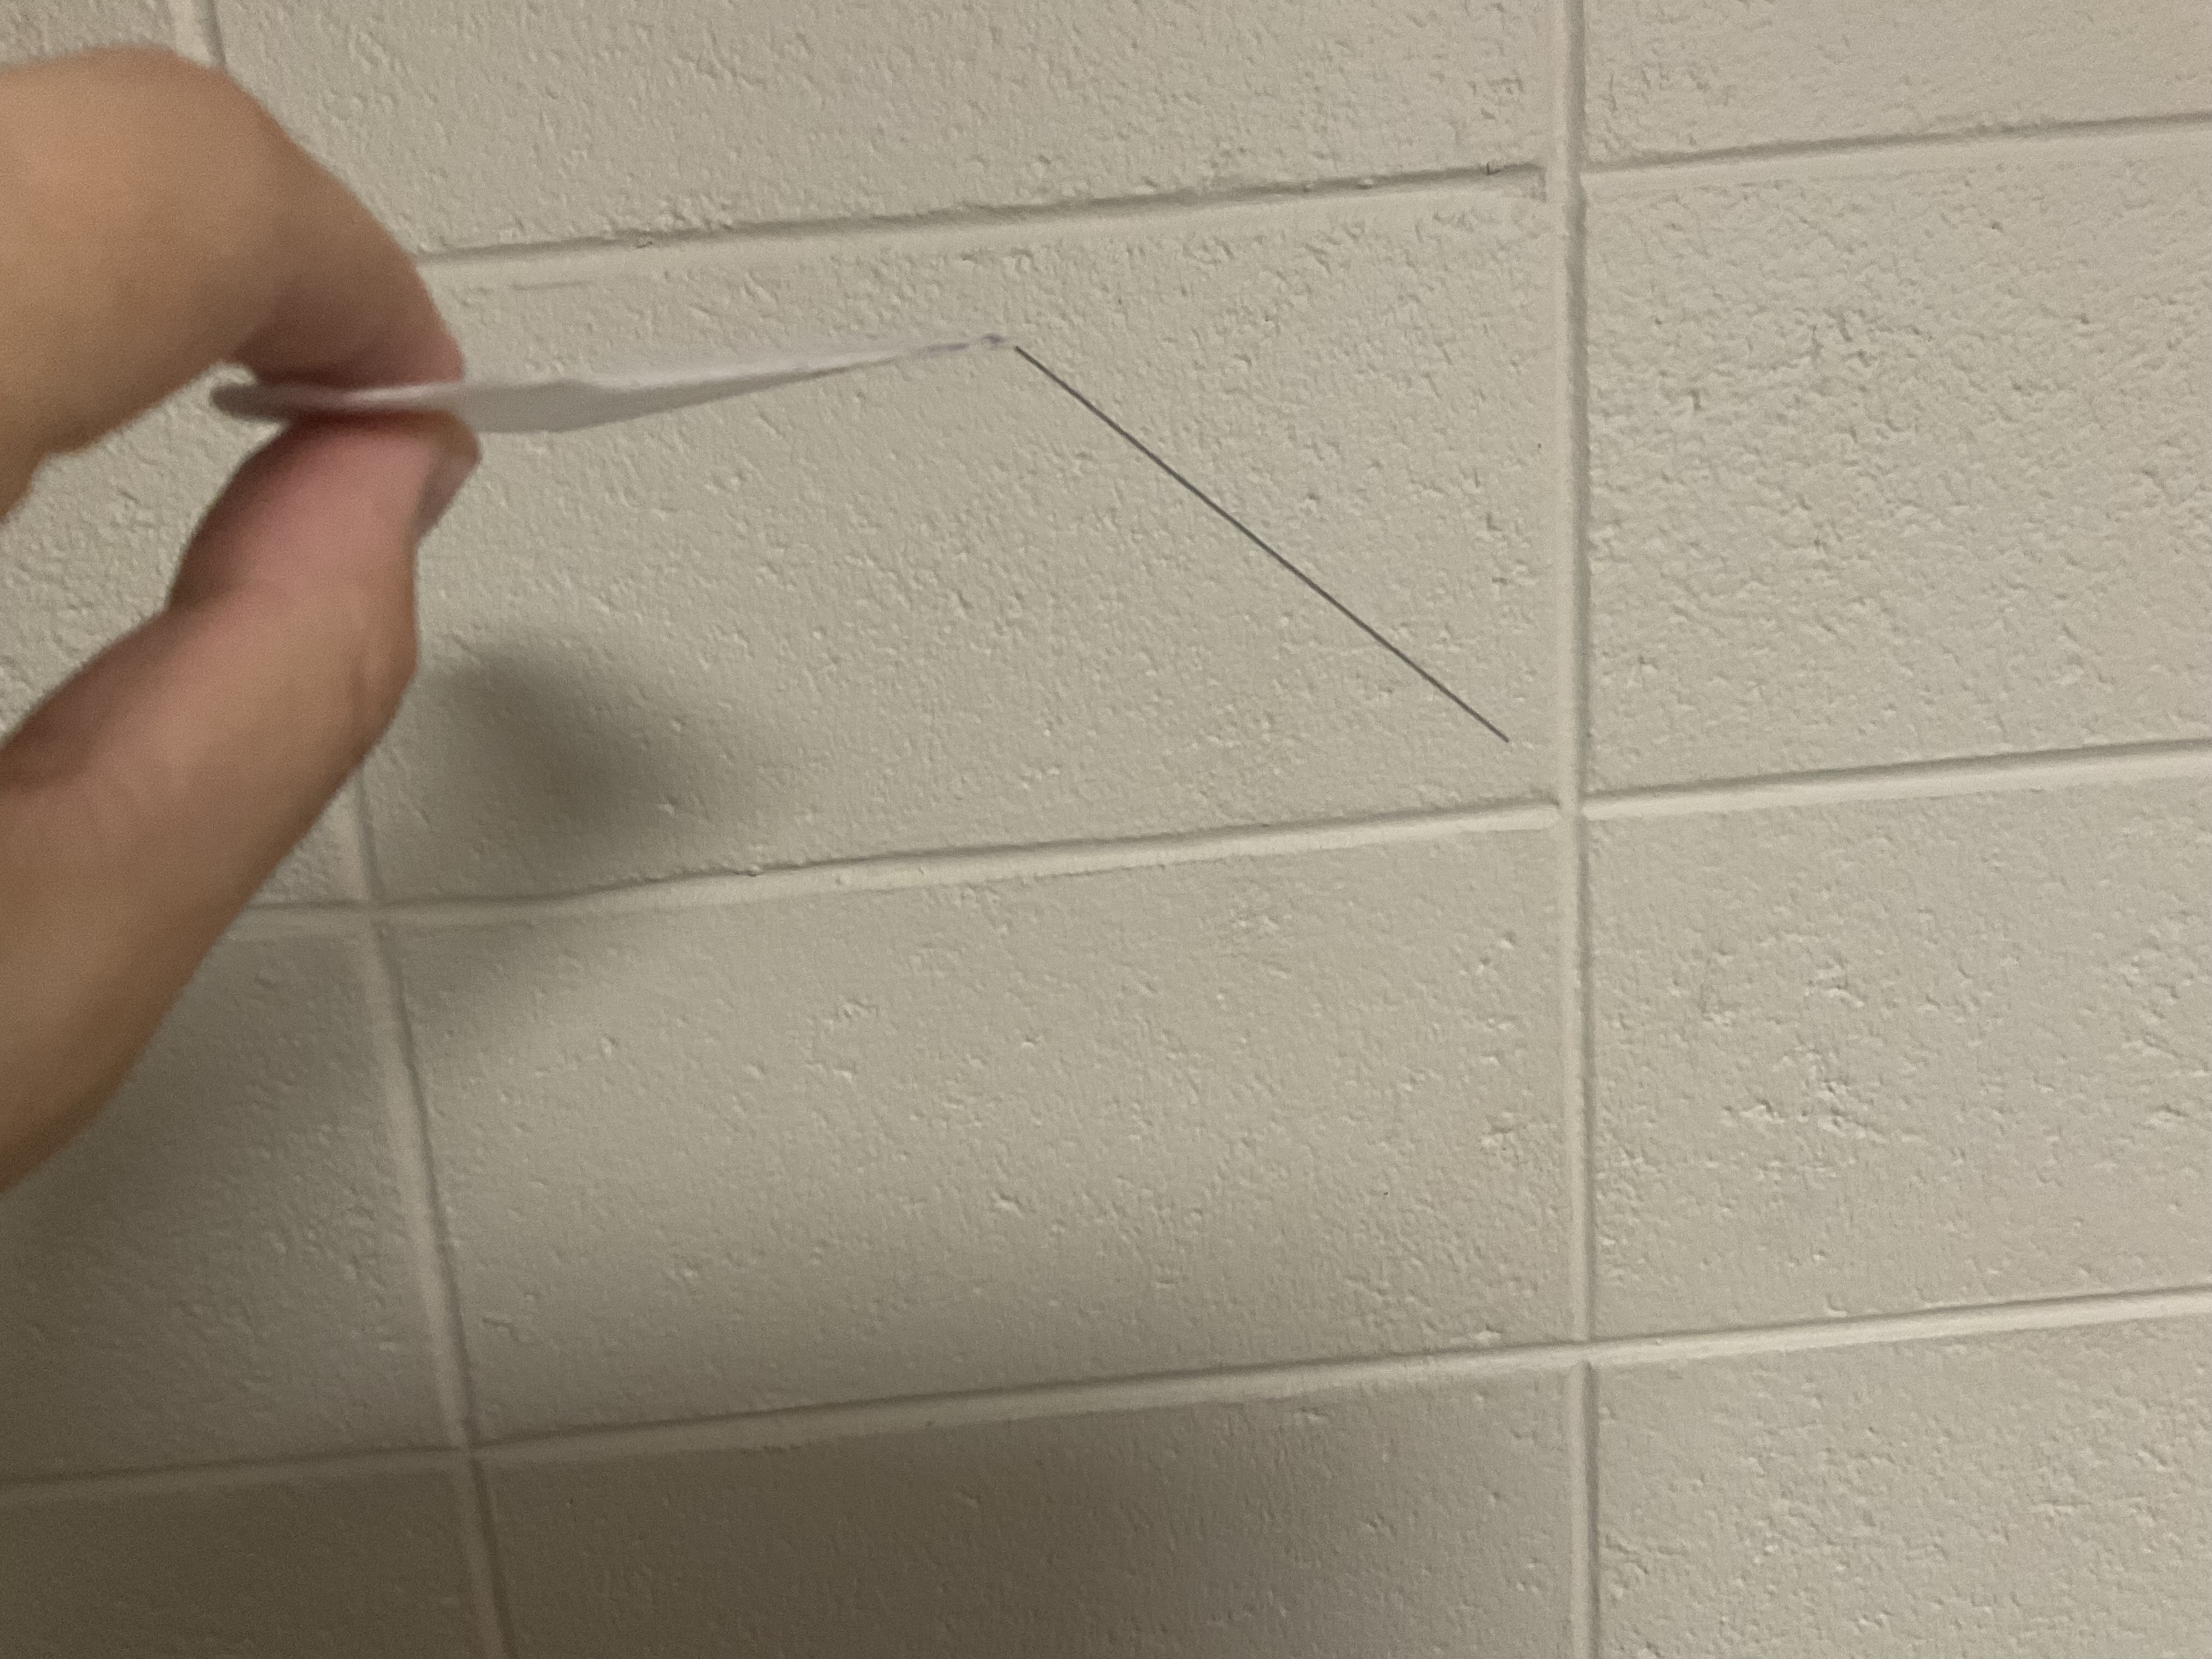
\includegraphics[width=0.5\linewidth]{IMG_3466.jpg}
    \caption{Forward CoM from front weight}
    \label{fig:placeholder}
\end{figure}

The reason for this is that with the CoM removed from the aerodynamic center, changes in lift and drag will be torques around the CoM. With the CoM in front of the aerodynamic center, an increase in lift will pitch the nose down, and a decrease will pitch the nose  up. In addition, if the nose pitches up, the projected area of the wing along the direction of travel will increase, increasing $C_{L}$ and increasing $L$, and of course the opposite happens when the nose pitches down. so with the CoM ahead of the dynamic center we see that we get a restoring reaction torque. Mathematically:

\begin{equation}
    M_{pitch,CoM} \approx d\times \frac{1}{2}\rho V^{2}S[C_L(\alpha)-C_L(\alpha_0)]
\end{equation}

for small changes in $\alpha$ where $d$ is the horizontal between the CoM and the aerodynamic center, $\alpha$ is the pitch angle, $\alpha_0$ is the equilibrium pitch angle, and $C_L$ is some increasing function of alpha. The change in Lift coefficient is small compared to that of the lift coefficient.

The other design consideration for pitch control is the trailing-edge camber.

\begin{figure}[h!]
    \centering
    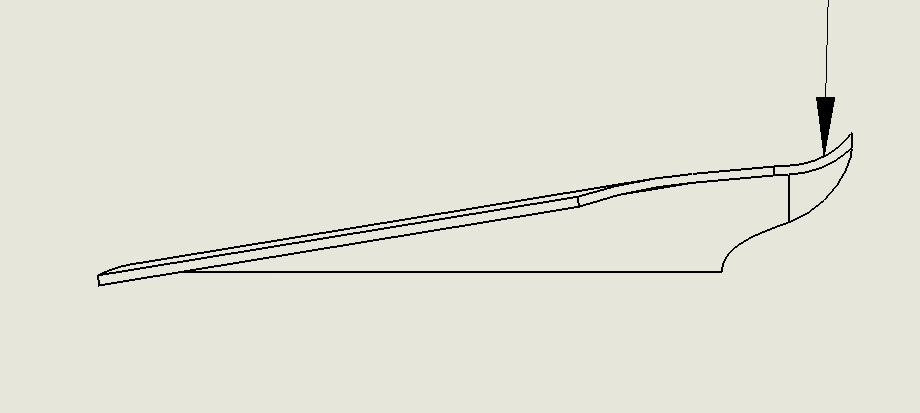
\includegraphics[width=0.7\linewidth]{Screenshot 2026-05-08 172751.png}
    \caption{trailing-edge camber with arrow}
    \label{fig:placeholder}
\end{figure}

The trailing-edge camber increases the drag force at the trailing edge of the glider. this increased drag force imparts a torque around the low and forward CoM without interfering with the lift of the glider. This drag helps to slow the glider down, and also keeps nose of the glider up, increasing the gliding pitch angle allowing the glider to expose more of its underside to the incoming air to increase lift and decrease the glide ratio and glide angle.

\subsubsection*{5.24 Reducing separation and the transition to turbulence}

As previously mentioned, due to the Reynolds number regime in which our glider is operating, it is crucial that we pay special attention to separation and the onset of turbulence. Over the course of iterating our design, we noticed that as we reduced the weight of our glider, it became more and more susceptible to fluttering. Gliders would struggle to enter an equilibrium glide, or would enter equilibrium for a short time before picking up an instability and falling out of the sky. The the change that finally got the lightest gliders to work was turning down the front edge. The explanation for why this worked is that we locally aligned the angle of attack of the craft with the streamline of the air. This change allowed for a smoother transition and redirection of the airflow over the wing, which is of course necessary for flight. 

\begin{figure}[h!]
    \centering
    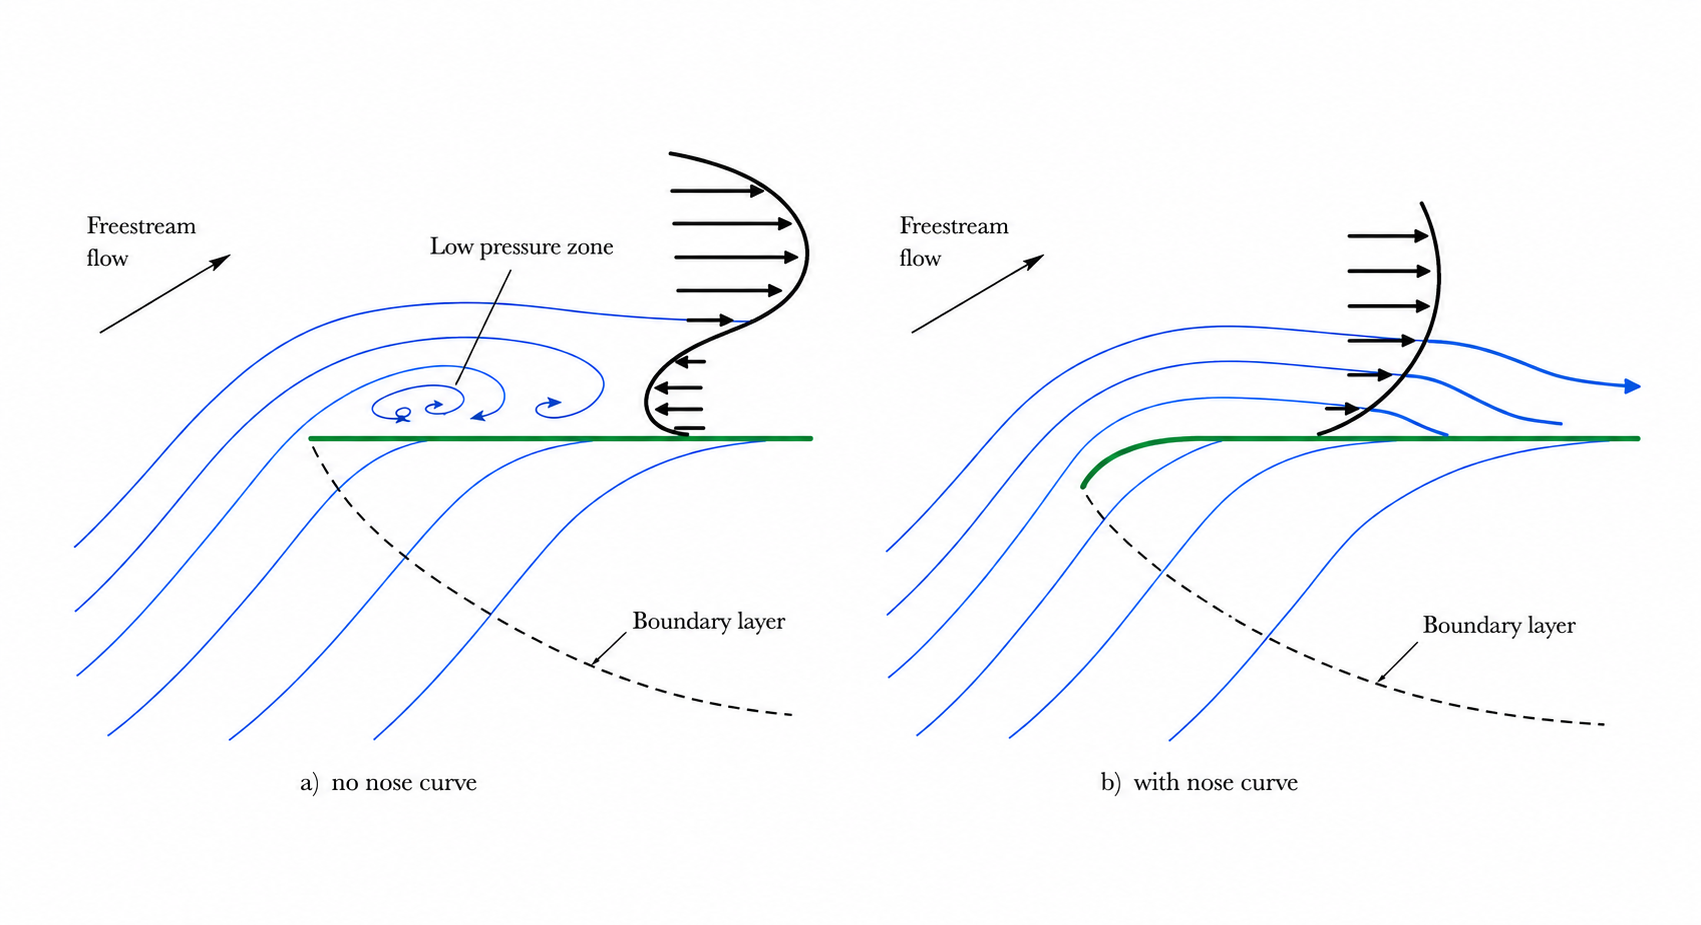
\includegraphics[width=1\linewidth]{image0.png}
    
    \label{fig:placeholder}
\end{figure}

As we can see from the figure on the right, the abrupt edge of the airfoil can create a zone of lower pressure, and because of our low Reynolds number, the flow close to the airfoil has very low momentum, and this low pressure easily separates the flow and you get regions where the air is flowing backwards along the airfoil. these disturbances can propagate downstream making the glider unflyable. In contrast, we can see that on the right, the flow gradually meets the curving airfoil and slowly adapts to its shape.  This ensures a more consistent pressure distribution which allows the glider to generate lift and fly. 


% PAGE 7
\pagehead{6. Experimental Results and Coefficient Extraction}

\subsection*{6.1 Video measurement method}
The glider's performance was estimated from video frames. A vertical drop of 18 inches and a horizontal travel distance of 90 inches gave
\begin{equation}
\tan\gamma=\frac{18}{90}=0.20, \qquad \gamma=\tan^{-1}(0.20)=11.3^\circ.
\end{equation}
The measured glide speed was $V=2.2$ m/s for the final light model. With $m=0.94$ g, $S=0.011$ m$^2$, and air density near $\rho=1.2$ kg/m$^3$, the steady-glide equations produce the reported lift and drag coefficients.

\begin{center}
\begin{tabular}{lcc}
\toprule
Quantity & Final light model & Heavier comparison model \\
\midrule
Mass $m$ & 0.94 g & 1.68 g \\
Projected area $S$ & 0.011 m$^2$ & 0.011 m$^2$ \\
Chord Length $c$ & 0.0635 m & 0.0635 m \\
Glide slope $\tan\gamma$ & 0.20 & 0.25 \\
Glide speed $V$ & 2.2 m/s & 2.8 m/s \\
Lift coefficient $C_L$ & 0.265 & 0.558 \\
Drag coefficient $C_D$ & 0.0531 & 0.140 \\
$\Rey$ & $9.4\times10^3$ & $1.2\times10^4$ \\
\bottomrule
\end{tabular}
\end{center}

\begin{figure}[h!]
    \centering
    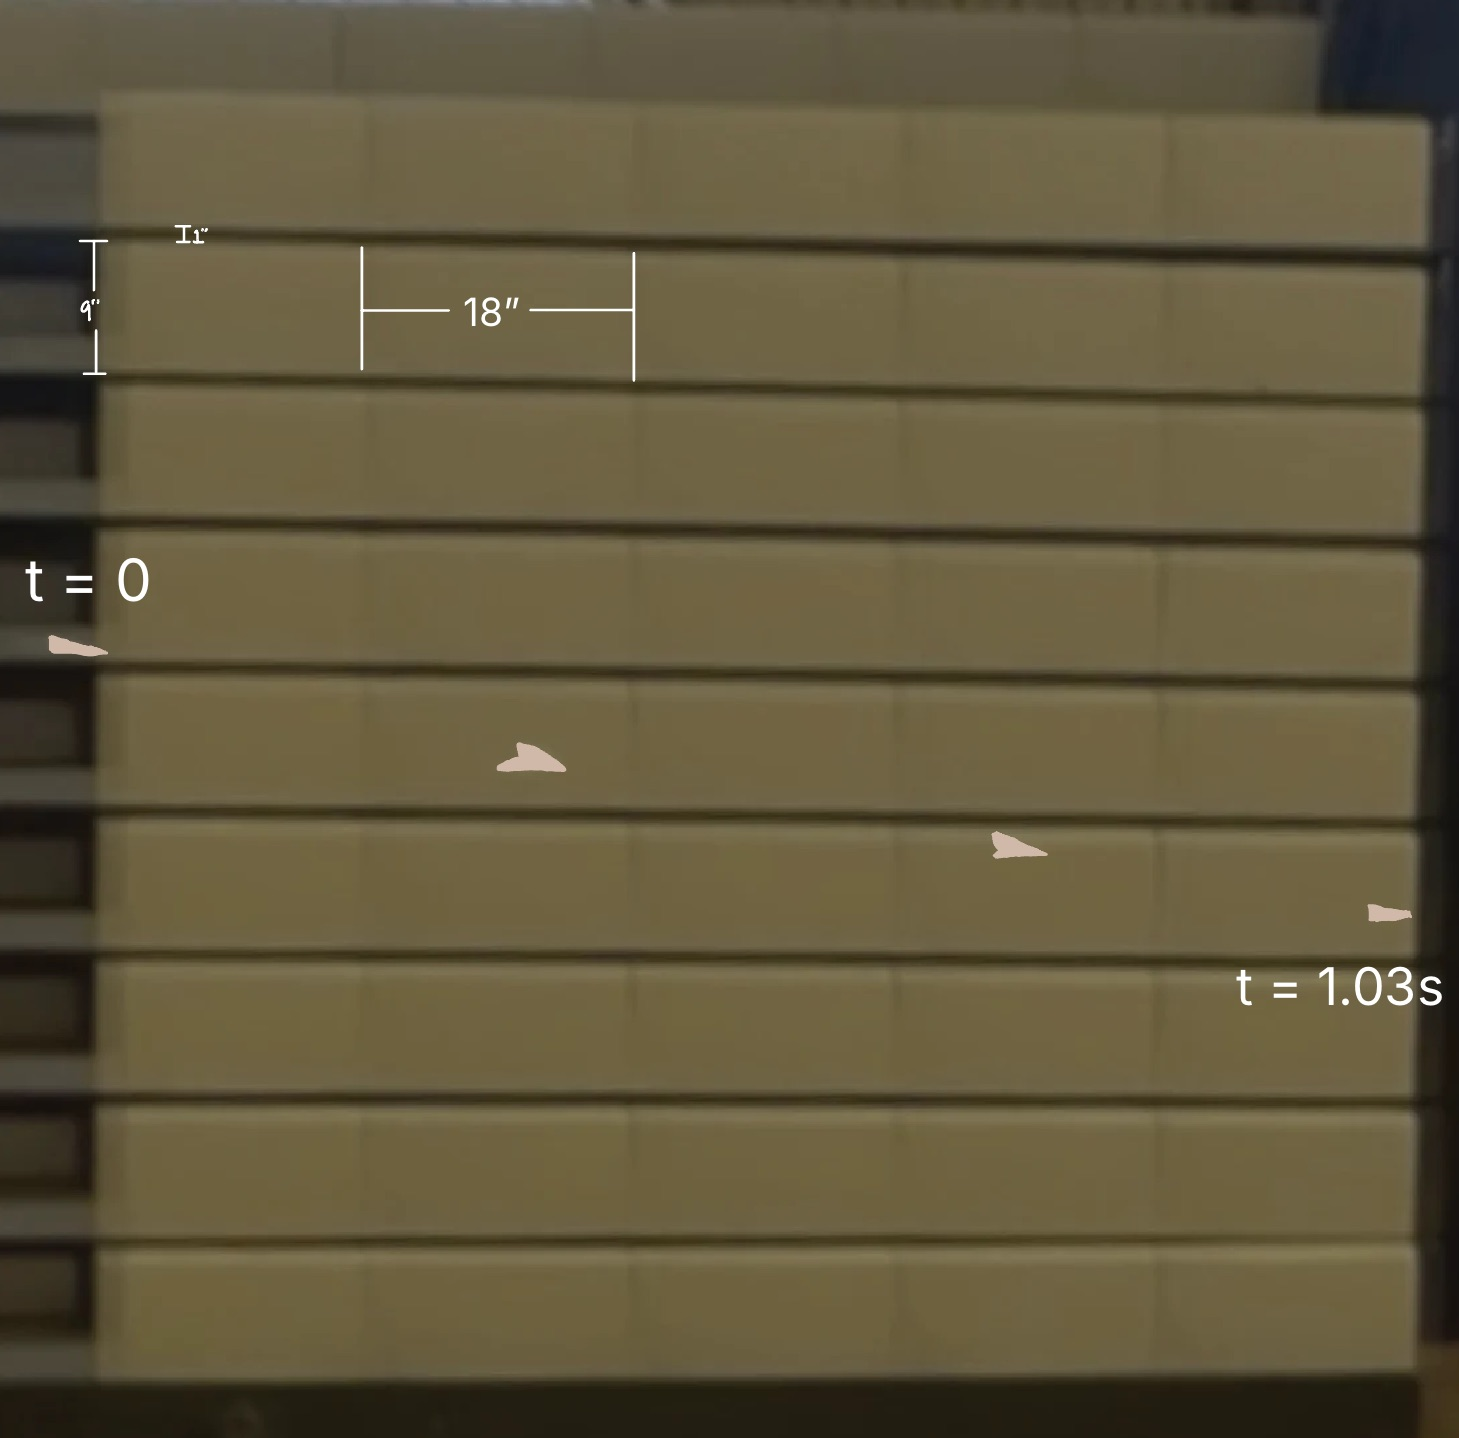
\includegraphics[width=0.5\linewidth]{NBMetadataCache.jpeg}
    \caption{Overlayed photos of test glide}
    \label{fig:placeholder}
\end{figure}

\subsection*{6.2 Interpretation of the light model}
For the final light glider,
\begin{equation}
\frac{L}{D}=\frac{1}{\tan\gamma}=5.0.
\end{equation}

With a glide speed of 2.2 m/s, and a Glide ratio of 5:1, the glider was entirely able to be flown at a walking pace, with the use of just ones hands, or even without ones hands, using instead ones head to generate the requisite upwash

\subsection*{6.3 Comparison to the heavier model}
The heavier model had the same projected area but nearly 1.8 times the mass. It flew at $2.8$ m/s rather than $2.2$ m/s and descended at a steeper glide slope. This is consistent with the theoretical scaling: increasing $m/S$ increases required dynamic pressure. The heavier model therefore required either a faster user or a stronger upwash surface. In testing, it required a sort of speed-walk-jog pace and a higher-surface object to generate enough upward flow. The heavier model also had a lift coefficient of more than double the lighter model. This likely due in part to the steeper glide angle which changed the angle of attack of the glider. It is also likely that due to higher reynolds number coming from the increased pace, the flow was able to stay attached to the wing better.

\subsection*{6.4 Experimental uncertainty}
The main sources of uncertainty were video perspective, frame-rate limits, manual identification of glider position, and the difference between still-air glide measurements and forced walkalong conditions. The coefficients should therefore be treated as engineering estimates rather than high quality experimental values. Still, the comparison between the light and heavy models is robust because the trend is clear: adding mass increased speed, sink demand, but also stability.



% PAGE 8
\pagehead{7. COMSOL Simulation and Comparison}

\subsection*{7.1 Simulation goal}
The simulation work was intended to test whether the final airfoil shape generated lift and drag values comparable to experiment, and to study how angle of attack and nose pitch affected pressure distribution and flow attachment. The CAD airfoil was placed into a COMSOL fluid model using the experimental airspeed and glide angle as reference conditions.

\subsection*{7.2 Baseline comparison}
The COMSOL baseline case predicted
\begin{equation}
C_L \approx 0.512, \qquad C_D \approx 0.008.
\end{equation}
Compared with the experimental values $C_L\approx0.265$ and $C_D\approx0.0531$, the simulation overpredicted lift and underpredicted drag. This discrepancy is plausible because the simulation idealizes the geometry, surface finish, flow field, and boundary conditions. Real EPS foam has imperfections, the hand-built glider may not be perfectly symmetric, and the walking upwash is unsteady and three-dimensional.

\begin{center}
\begin{tabular}{lccc}
\toprule
Case & $C_L$ & $C_D$ & Interpretation \\
\midrule
Experiment, final glider & 0.265 & 0.0531 & Includes real drag, asymmetry, and unsteady effects \\
COMSOL baseline & 0.512 & 0.008 & More idealized, cleaner attached-flow prediction \\
\bottomrule
\end{tabular}
\end{center}

\subsection*{7.3 Angle-of-attack sweep}
The simulation swept angle of attack through 0$^\circ$, 5$^\circ$, 11$^\circ$, 15$^\circ$, and 20$^\circ$. The general trend was an increase in lift with angle of attack, but the important issue was not only the scalar value of $C_L$. The pressure and velocity fields showed how high angle of attack can strengthen suction on the upper surface while also increasing risk of separation, especially near tips and leading-edge regions.

\begin{center}
\begin{tabular}{cccc}
\toprule
$\alpha$ (rad) & $\alpha$ (deg) & $C_L$ & $C_D$ \\
\midrule
0.00000 & 0 & 0.176 & 0.042 \\
0.08727 & 5 & 0.486 & 0.052 \\
0.19199 & 11 & 0.512 & 0.009 \\
0.26180 & 15 & 0.674 & -0.003 \\
0.34907 & 20 & 0.802 & -0.011 \\
\bottomrule
\end{tabular}
\end{center}
\begin{figure}[h!]
    \centering
    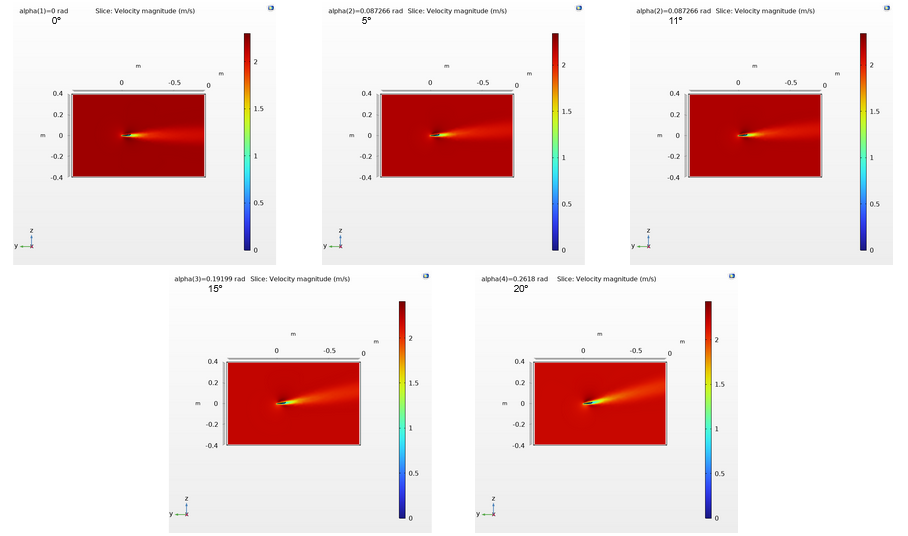
\includegraphics[width=0.75\linewidth]{velocityprofile1.png}
    \caption{Velocity profile as $\alpha$ changes}
    \label{fig:velocityprofile}
\end{figure}
The negative or very small drag coefficients in some simulated cases should not be interpreted as physically reliable predictions of free-flight performance. They indicate that the model setup and force integration are sensitive to boundary conditions and pressure references. This can also be interprested in the real world as high angles of attack in planes lead them to stall and hence its a prediction that our glider wouldn't fly at those angles. For comparison with experiment, the qualitative flow structure and relative changes with geometry are more reliable than absolute drag values.

The heavier model produced a measured lift coefficient experimentally closer to the COMSOL prediction. This agreement should not be interpreted as a purely geometric improvement, because the heavier glider also flew under a different operating condition. Its larger weight required a higher flight speed and a steeper glide angle, which changed the effective angle of attack. Since lift coefficient is strongly dependent on angle of attack, even a small change in trim condition can move the experimental result closer to the simulated value.

A second possible explanation is improved flow attachment at higher Reynolds number. The heavier glider flew at approximately \(V=2.8~\mathrm{m/s}\), compared to \(V=2.2~\mathrm{m/s}\) for the lighter glider. This increase in speed raises the Reynolds number and may reduce the severity of low-Reynolds-number separation effects. In the low-\(Re\) regime, the boundary layer is sensitive to small perytubations, surface roughness, and local leading-edge geometry. A slightly higher Reynolds number can delay separation or allow partial reattachment, causing the real flow field to resemble the idealized COMSOL solution more closely.

Therefore, the closer agreement between the heavier model and COMSOL likely reflects both angle-of-attack differences and Reynolds-number effects. However, this came at the cost of walkalong performance: the heavier model required a faster walking speed and stronger upwash, making it harder to sustain compared with the lighter glider.

\subsection*{7.4 Pressure distribution and tip behavior}
The pressure comparison between a pitched-down tip and a straight tip suggested why tip geometry mattered. The pitched-down tip maintained a more uniform low-pressure region across the upper surface and a spanwise high-pressure region underneath. The straight tip showed pressure recovery near the tips, creating a path for high-pressure air to leak around the tip and reduce local lift. At low Reynolds number, this can strongly affect the entire small wing.
\begin{figure}[h!]
    \centering
    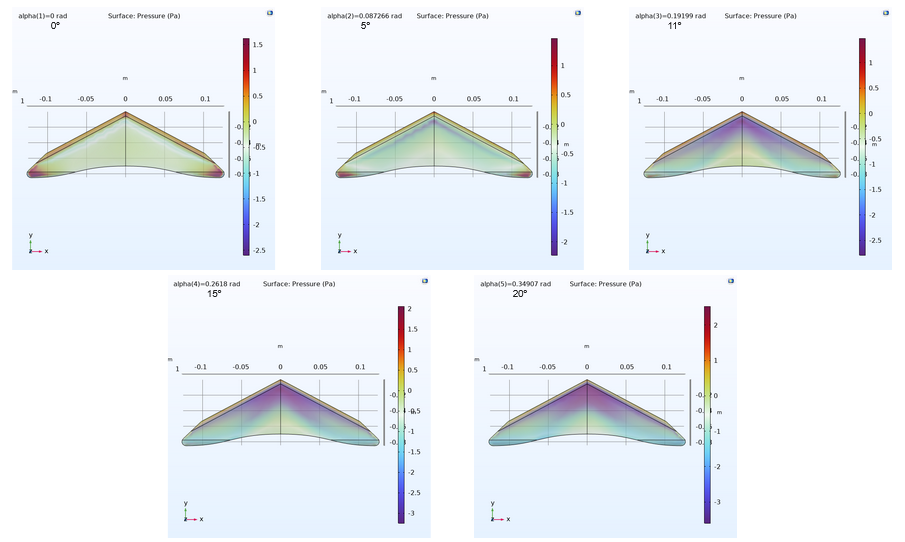
\includegraphics[width=0.75\linewidth]{pressuregradient.png}
    \caption{Pressure Distribution as $\alpha$ changes}
    \label{fig:pressuregrad}
\end{figure}
\newpage

% PAGE 9
\pagehead{8. Nose Pitch, Separation, and Stability Simulations}

\subsection*{8.1 Why nose pitch matters}
The leading portion of the airfoil is where the boundary layer first forms. If the local surface angle is too aggressive relative to the incoming flow, the flow separates early. Once separated, the upper-surface suction is reduced, pressure drag increases, and the glider can flutter or pitch unpredictably. A slight nose-down or flow-aligned entry reduces the effective local angle of attack at the nose while allowing the aft camber to maintain overall lift and pitch trim. This phenomenon was explained in detail in the section 5.24. 

\begin{figure}[h!]
    \centering
    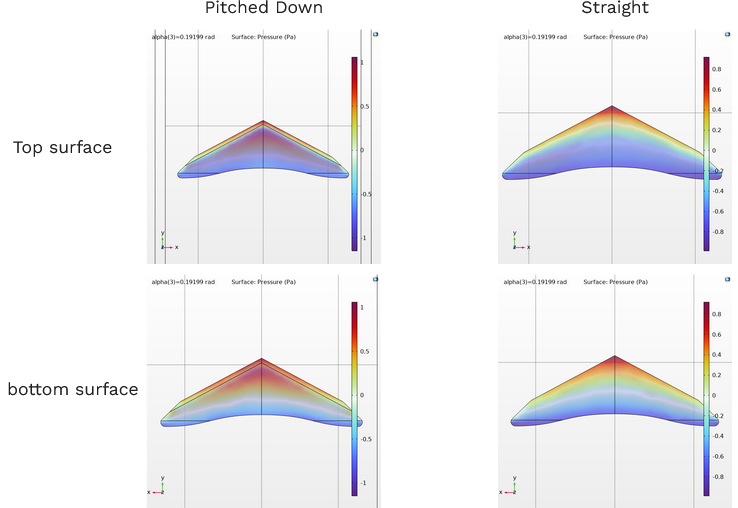
\includegraphics[width=0.5\linewidth]{straightvsnose.png}
    \caption{Pressure distribution with pitched down wing vs. straight wing}
    \label{fig:pressure}
\end{figure}

\subsection*{8.2 Pressure distribution comparison}

The pressure plots show why the pitched-down nose geometry was more stable than the straight leading-edge configuration. In the pitched-down case, the upper surface maintains a more uniform low-pressure region across the span. This indicates that the wing is producing lift more consistently from the centerline out toward the tips. The bottom surface also maintains a relatively continuous high-pressure region, so the pressure difference between the upper and lower surfaces remains strong over most of the wing.

In contrast, the straight configuration shows stronger pressure recovery near the tips. This means the tips contribute less effectively to lift, because the pressure difference between the top and bottom surfaces weakens locally. The straight wing also creates a more direct high-pressure-to-low-pressure leakage path around the tip, which promotes tip vortex formation and increases induced drag. At the low Reynolds numbers, this effect is especially important because the flow is more sensitive to small changes in surface angle and geometry.

The pitched-down nose therefore improves performance in two connected ways. First, it helps align the incoming flow with the local leading-edge surface, delaying separation and reducing flutter. Second, it preserves a cleaner pressure differential across the span, which improves lift generation and roll stability. This is why the final design used a slight nose-down leading-edge shape combined with aft camber: the front geometry helped keep the flow attached, while the rear camber helped maintain the positive pitching moment needed for trim.\newpage

% PAGE 10
% PAGE 10
\pagehead{9. Conclusion and Future Work}

\subsection*{9.1 Conclusion}

This project showed that a walkalong glider is not just a small version of a conventional airplane. Because it operates at walking speed and low Reynolds number, its performance is controlled by a coupled balance between weight, lift generation, pitch trim, roll stability, and flow attachment. The final working glider succeeded because it combined very low mass, a forward and low center of mass, aft camber, dihedral, and a slightly nose-down leading-edge shape.

Experimentally, the final light model had a mass of \(0.94~\mathrm{g}\), projected area of \(0.011~\mathrm{m^2}\), glide speed of \(2.2~\mathrm{m/s}\), and glide ratio of approximately \(5:1\). These values made it slow enough to remain in the upwash generated by a walking person. The heavier comparison model generated a lift coefficient closer to the COMSOL prediction, but it required a higher speed and stronger upwash, making it less practical for actual walkalong flight.

The simulations helped explain the design behavior observed during testing. In particular, the pitched-down nose geometry produced a more favorable pressure distribution and appeared to reduce separation near the leading edge and tips. This supported the experimental observation that small changes in nose shape had a large effect on stability and glide quality. Overall, the project demonstrated that successful walkalong flight depends less on maximizing lift alone and more on achieving a stable, low-speed, attached-flow operating condition.

\subsection*{9.2 Future Work}

Future work could improve both the experimental measurements and the simulation model. The most useful next step would be to collect more accurate flight data using a fixed camera setup, calibrated background grid, and frame-by-frame tracking of position, pitch angle, and velocity. This would reduce uncertainty in the glide speed, glide ratio, and extracted lift and drag coefficients.

A second improvement would be to directly measure or visualize the walker-generated upwash field. Smoke visualization, lightweight streamers, or particle tracking could show where the useful upwash region forms and how the glider moves within it. This would make it possible to connect the forced-flow state-vector model more directly to the physical walking experiment.

The COMSOL model could also be extended. A more complete simulation would include three-dimensional flow, a moving upstream board or hand, surface roughness, and unsteady flow effects. This would likely improve the comparison between simulated and experimental drag. Additional parameter sweeps over nose pitch, camber, dihedral angle, and center-of-mass location would also help identify an optimal geometry rather than relying mainly on manual iteration.

Finally, future prototypes could test more controlled construction methods. Laser-cut templates, thinner foam stock, adjustable nose weights, and repeatable camber-forming fixtures would make it easier to isolate individual design variables. This would allow a more systematic study of how each geometric feature contributes to stable walkalong flight.

\subsection*{References}
\begin{enumerate}[label={[\arabic*]}]
\item ScienceToyMaker. \textit{Walkalong glider resources and build references}. Available at \url{http://sciencetoymaker.org}.
\item Alblas, D., van den Bosch, M., Feigl, Z., Klomp, L., Rottschafer, V., Schwenninger, F., Spek, L., Weedage, L., and Zeijlemaker, S. \textit{A Joint Data- and Model-Driven Approach Simulating the Behaviour of a Walkalong Glider}. 2023. DOI: 10.33774/miir-2023-p957p.
\end{enumerate}
\end{document}
